%!TEX program = xelatex
\documentclass[11pt, a4paper]{article}
	\usepackage[a4paper,top=3cm,bottom=4cm,left=2.5cm,right=2.5cm]{geometry}
	\usepackage{graphicx}
	\graphicspath{{../images/}}
	\usepackage{hyperref}
	\usepackage{xepersian}
	\settextfont[Scale=1.2]{B Nazanin}
	\setlatintextfont[Scale=1]{Times New Roman Cyr}
    \title{\textbf{شبیه‌سازی رایانه‌ای در فیزیک}
    \\تمرین اول: \lr{Cellular Automata}}
    \author{سینا معمر ۹۵۱۰۲۳۱۶}
    

\begin{document}

\maketitle
\thispagestyle{empty}


\section{\textbf{قانون کلاه}}
\subsection{اتوماتای سلولی یک بعدی}
\paragraph{}
از آنجایی که سوالات ۱ تا ۳ همگی در دسته‌ی \lr{cellular automata} های یک بعدی قرار می‌گیرند و تنها در شرایط اولیه، زمان و قانون تفاوت دارند، کلاس \lr{CA1D} در فایل \lr{automata.py} پیاده‌سازی و در این ۳ سوال از این کلاس استفاده شده است. در زیر به تشریح ساختار و عملکرد این کلاس می‌پردازیم.\\
برای ساخت یک \lr{object} از این کلاس به دو ورودی "تعداد سلول‌ها" و "شرایط اولیه نیاز" است. برای ایجاد شرایط اولیه تصادفی از \lr{"rand"} استفاده و در غیر این صورت باید لیستی از شماره‌ی خانه‌های روشن فرستاده شود. برای ذخیره وضعیت سلول‌ها از کلاس \lr{bitarray} استفاده می‌کنیم تا تنها یک بیت از حافظه برای هر سلول اشغال شود.\\
برای انجام شبیه‌سازی تابع \lr{render} را باید صدا بزنیم. برای این کار به "شماره قانون" و "زمان" نیاز داریم. شیوه کار این تابع به این صورت است که ابتدا با استفاده از تابع \lr{\_\_LUT\_\_} یک دیکشنری از ۸ حالت ممکن برای همسایگی‌ها و وضعیت بعدی سلول متناظر با آن‌ها می‌سازیم. به این صورت که شماره قانون را به مبنای ۲ برده و لیست حاصل شده را پیمایش می‌کنیم و نتیج را به صورت \lr{\{key, value\}} به \lr{LUT} اضافه می‌کنیم. در ادامه‌ی تابع \lr{render}، روی لیست سلول‌ها پیمایش می‌کنیم و وضعیت همسایه‌های آن را به صورت یک عدد ۳ رقمی در مبنای ۲ به یک \lr{string} تبدیل کرده و به این طریق \lr{key} معادل با وضعیت بعدی سلول در \lr{LUT} مان را به دست می‌آوریم و لیست سلول‌های جدید را می‌سازیم و به لیست \lr{grids} اضافه می‌کنیم.\\
در پایان برای نمایش عکس حاصل، تابع \lr{show} را فراخوانی می‌کنیم. این تابع برای نمایش عکس از لیست سلول‌های ما، ابتدا وضعیت هر سلول را به \lr{Not} آن تبدیل می‌کند تا سلول‌های روشن به رنگ سیاه نمایش داده بشوند. سپس تابع \lr{imshow} از کتاب‌خانه \lr{matplotlib} صدا زده می‌شود.
\subsection{مسئله گسترش رفتار}
\paragraph{}
مسئله‌ی گسترش رفتار یک نمونه از \lr{CA} یک بعدی است. طبق گفته مسئله، هر سلول تنها در صورتی در مرحله بعدی روشن خواهد بود که تنها یکی از همسایه‌های چپ و راستش روشن باشند، یعنی یکی از حالت‌های روبرو: \lr{\{100, 110, 001, 011\}}. و در باقی حالات، خاموش خواهد بود.


\begin{table}
	\begin{center}
		\begin{tabular}{|c c c c c c c c|} 
		\hline
		\lr{000} & \lr{001} & \lr{010} & \lr{011} & \lr{100} & \lr{101} & \lr{110} & \lr{111} \\ [0.5ex] 
		\hline
		\lr{0} & \lr{1} & \lr{0} & \lr{1} & \lr{1} & \lr{0} & \lr{1} & \lr{0} \\ 
		\hline
		\end{tabular}
	\end{center}
	\caption{قانون مسئله گسترش رفتار}
	\label{tab:q1-rule}
\end{table}



در نتیجه همان طور که در جدول \ref{tab:q1-rule} مشاهده می‌شود، قانون ما $(01011010)_2$ یا همان ۹۰ خواهد بود. همچنین ۲۰۱ سلول داریم که در زمان ۰ تنها سلول ۱۰۱ روشن است. برای نشان دادن پخش شدن این مد در جامعه، ۲۰۰ واحد زمانی آن را بررسی می‌کنیم. کد این بخش از سوال در فایل \lr{q1.py} قابل مشاهده است.\\

\begin{figure}[h]
    \centering
    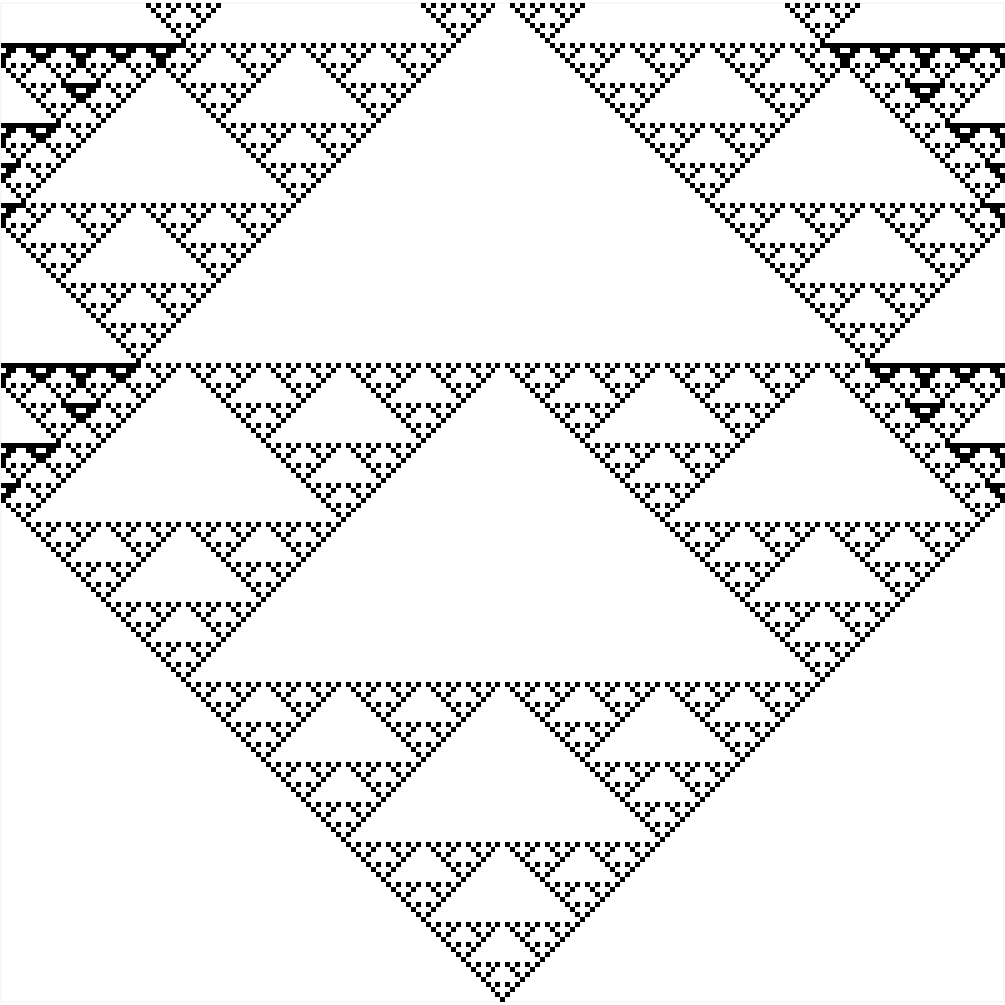
\includegraphics[width=0.5\textwidth]{q1}
    \caption{اتوماتای سلولی یک بعدی به طول ۲۰۱ با قانون ۹۰ و ۲۰۰ دوره زمانی، شرایط اولیه: تنها خانه‌ی ۱۰۱ روشن}
    \label{fig:q1}
\end{figure}

همان طور که در شکل \ref{fig:q1} مشاهده می‌شود، چگونگی گسترش مد در این جامعه، مشابه مثلث سرپینسکی است. نکته قابل توجه این شکل آن است که چگونگی پخش شدن مد در هر اسکیلی، مشابه با چگونگی پخش شدن مد در اسکیل‌های کوچک‌تر همان جامعه است که کاملا متناسب با توقع ما از مسئله است.



\section{\textbf{قوانین ۲۵۶گانه}}
\paragraph{}
برای این سوال نیز همانند بخش قبل عمل می‌کنیم و از کلاس \lr{CA1D} استفاده می‌کنیم. شرایط اولیه هر دو یکسان و به طول ۲۰۱ با تنها یک سلول روشن در وسط است. نمودار هر دو‌ی آن‌ها را برای ۲۰۰ واحد زمانی به دست می‌آوریم. نمودار قانون ۱۱۰ در شکل \ref{fig:q2-110} و نمودار قانون ۷۵ در شکل \ref{fig:q2-75} قابل مشاهده است.

\begin{figure}[!tbp]
  \centering
  \hfill
  \begin{minipage}[b]{0.4\textwidth}
    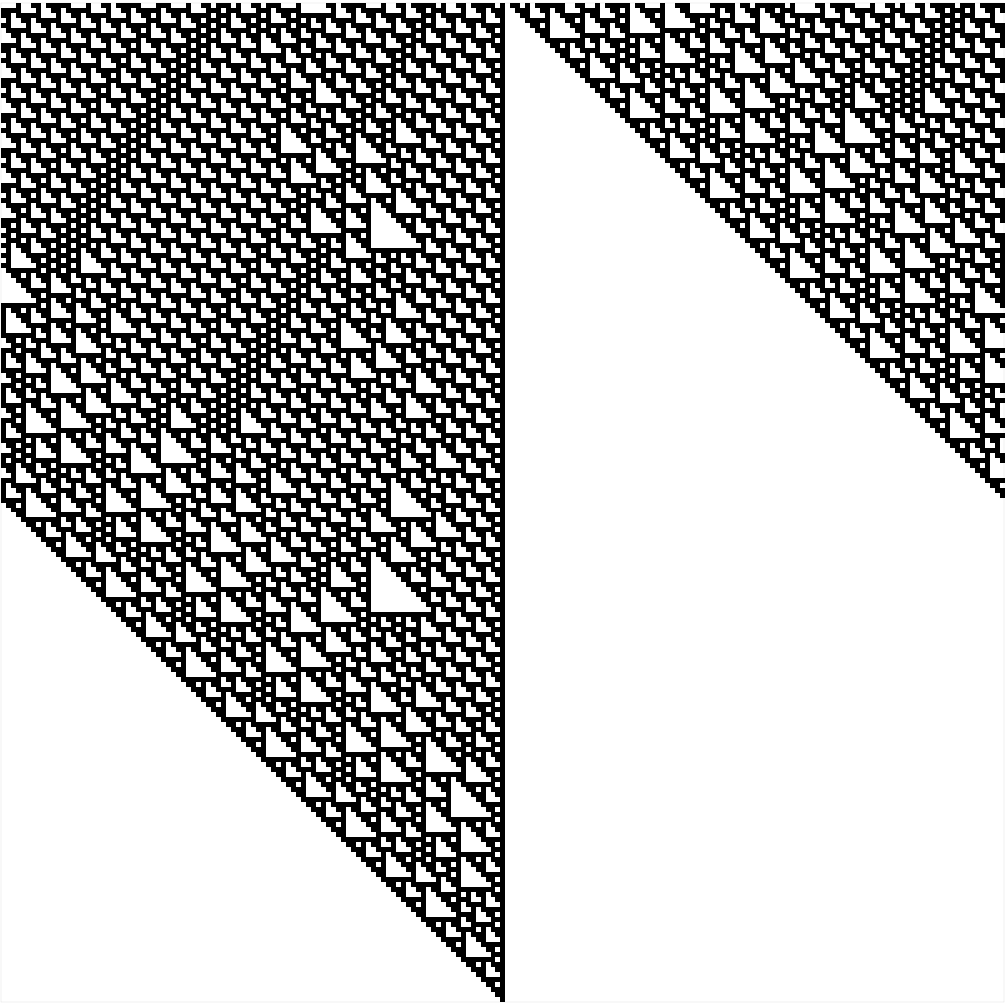
\includegraphics[width=\textwidth]{q2-110}
    \caption{اتوماتای سلولی یک بعدی به طول ۲۰۱ با قانون ۱۱۰ و ۲۰۰ دوره زمانی، شرایط اولیه: تنها خانه‌ی ۱۰۱ روشن}
    \label{fig:q2-110}
  \end{minipage}
  \hfill
  \begin{minipage}[b]{0.4\textwidth}
    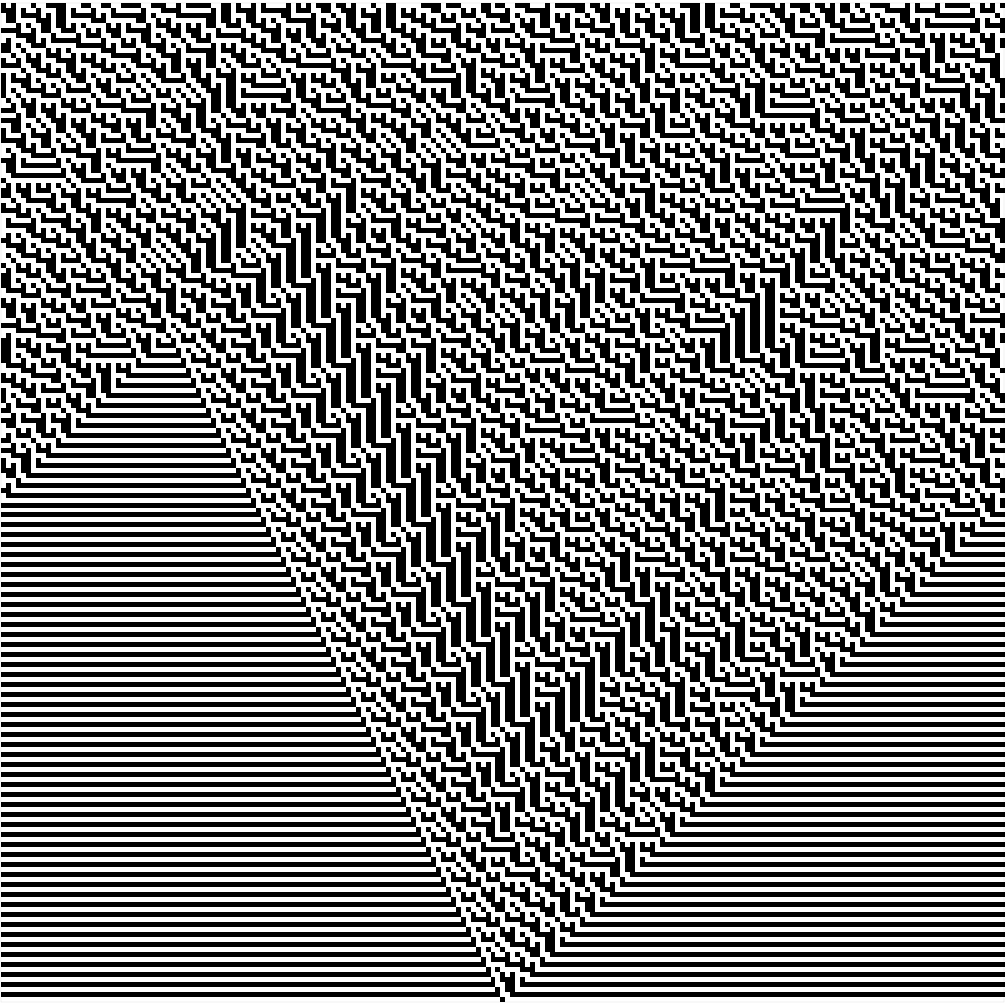
\includegraphics[width=\textwidth]{q2-75}
    \caption{اتوماتای سلولی یک بعدی به طول ۲۰۱ با قانون ۷۵ و ۲۰۰ دوره زمانی، شرایط اولیه: تنها خانه‌ی ۱۰۱ روشن}
    \label{fig:q2-75}
  \end{minipage}
  \hfill
\end{figure}

\subsection{بهینه‌سازی حافظه}
\paragraph{}
برای بهینه‌سازی حافظه، می‌توانیم از متغیر‌های \lr{boolean} و یا \lr{bit} برای ذخیره‌سازی وضعیت سلول‌ها استفاده کنیم تا تنها یک بیت از حافظه را به ازای هر سلول اشغال کنیم. همچنین می‌توان به جای ذخیره کردن وضعیت تمام سلول‌ها در هر مرحله، تنها شماره سلول‌هایی که وضعیت‌شان تغییر کرده است را ذخیره کنیم. که این‌ کار تحت شرایطی که تعداد سلول‌هایی که تغییر وضعیت داده‌اند کمتر از حد $\frac{N}{log_2 N}$ باشد، به کاهش حافظه کمک می کند ولی از طرف دیگر، پیچیدگی محاسبات و زمان اجرا را افزایش می‌دهد. علاوه بر این از آنجایی که در نهایت برای نمایش گرافیکی نیاز به لیستی از وضعیت تک تک سلول‌ها در هر مرحله داریم، پس عملا این کار بی‌تاثیر خواهد بود.

\section{\textbf{\lr{Wolfram Classification}}}
\paragraph{}
در این بخش نیز همانند بخش‌های پیشین، از کلاس \lr{CA1D} استفاده می‌کنیم. برای به دست آوردن شکل‌های ذکر شده در سوال، از شرایط اولیه‌ای به طول ۲۰۱ که تنها سلول مرکزی روشن باشد، استفاده می‌کنیم و ۳۰۰ واحد زمانی آن را روشن می‌گذاریم.\\
همچنین برای مشخص کردن دسته‌بندی‌ آن‌ها، باید از شرایط اولیه تصادفی شروع کنیم و بر اساس ظاهر و ویژگی‌های شکل به دست آمده، این کار را انجام دهیم.

\subsection{قانون ۴۶}
این قانون در مبنای ۲ به صورت $(00101110)_2$ است که با قانون $110=(01101110)_2$ تنها در رقم ۷ ام متفاوت است. نمودار حاصل از این قانون را در شکل \ref{fig:q3-46} مشاهده می‌کنیم.\\
همچنین برای دسته‌بندی کردن آن باید نمودار این قانون با شرایط اولیه تصادفی را هم داشته باشیم، که این نمودار را در شکل \ref{fig:q3-46-rand} می‌توان مشاهده نمود. همان طور که در شکل دیده می‌شود، طرح‌های به نسبت منظمی ولی به صورت تقریبا تصادفی شکل گرفته است. پس در کلاس ۴ قرار می‌گیرد.

\subsection{قانون ۷۸}
این قانون در مبنای ۲ به صورت $(01001110)_2$ است که با قانون $110=(01101110)_2$ تنها در رقم ۶ ام متفاوت است. نمودار حاصل از این قانون را در شکل \ref{fig:q3-78} مشاهده می‌کنیم.\\
همچنین برای دسته‌بندی کردن آن باید نمودار این قانون با شرایط اولیه تصادفی را هم داشته باشیم، که این نمودار را در شکل \ref{fig:q3-78-rand} می‌توان مشاهده نمود. همان طور که دیده می‌شود، به یک طرح ثابت و پایدار می‌رسیم. پس این قانون در کلاس ۲ قرار می‌گیرد.

\subsection{قانون ۱۰۲}
این قانون در مبنای ۲ به صورت $(01100110)_2$ است که با قانون $110=(01101110)_2$ تنها در رقم ۴ ام متفاوت است. نمودار حاصل از این قانون را در شکل \ref{fig:q3-102} مشاهده می‌کنیم.\\
همچنین برای دسته‌بندی کردن آن باید نمودار این قانون با شرایط اولیه تصادفی را هم داشته باشیم، که این نمودار را در شکل \ref{fig:q3-102-rand} می‌توان مشاهده نمود. همان طور که در شکل دیده می‌شود، طرح به دست آمده پیچیده است ولی در عین حال به طور نسبی دارای نویز کمی است و به طور موضعی تکرار می‌شوند. پس در کلاس ۴ قرار می‌گیرد. 

\subsection{قانون ۱۰۶}
این قانون در مبنای ۲ به صورت $(01101010)_2$ است که با قانون $110=(01101110)_2$ تنها در رقم ۳ ام متفاوت است. نمودار حاصل از این قانون را در شکل \ref{fig:q3-106} مشاهده می‌کنیم.\\
همچنین برای دسته‌بندی کردن آن باید نمودار این قانون با شرایط اولیه تصادفی را هم داشته باشیم، که این نمودار را در شکل \ref{fig:q3-106-rand} می‌توان مشاهده نمود. همان طور که در شکل دیده می‌شود، طرح به دست آمده پیچیده و تصادفی و همراه با نویز بسیار است. پس در کلاس ۳ قرار می‌گیرد.

\subsection{قانون ۱۰۸}
این قانون در مبنای ۲ به صورت $(01101100)_2$ است که با قانون $110=(01101110)_2$ تنها در رقم ۲ ام متفاوت است. نمودار حاصل از این قانون را در شکل \ref{fig:q3-108} مشاهده می‌کنیم.\\
همچنین برای دسته‌بندی کردن آن باید نمودار این قانون با شرایط اولیه تصادفی را هم داشته باشیم، که این نمودار را در شکل \ref{fig:q3-108-rand} می‌توان مشاهده نمود. همان طور که در شکل دیده می‌شود، طرح به دست آمده به دو الگو ثابت که به طور تناوبی تکرار می‌شوند، می‌رسد. پس در کلاس ۲ قرار می‌گیرد.

\subsection{قانون ۱۱۱}
این قانون در مبنای ۲ به صورت $(01101111)_2$ است که با قانون $110=(01101110)_2$ تنها در رقم ۱ ام متفاوت است. نمودار حاصل از این قانون را در شکل \ref{fig:q3-111} مشاهده می‌کنیم.\\
همچنین برای دسته‌بندی کردن آن باید نمودار این قانون با شرایط اولیه تصادفی را هم داشته باشیم، که این نمودار را در شکل \ref{fig:q3-111-rand} می‌توان مشاهده نمود. همان طور که در شکل دیده می‌شود، طرح‌های به نسبت منظمی ولی به صورت تقریبا تصادفی شکل گرفته است. پس در کلاس ۴ قرار می‌گیرد.

\subsection{قانون ۱۲۶}
این قانون در مبنای ۲ به صورت $(01111110)_2$ است که با قانون $110=(01101110)_2$ تنها در رقم ۵ ام متفاوت است. نمودار حاصل از این قانون را در شکل \ref{fig:q3-126} مشاهده می‌کنیم.\\
همچنین برای دسته‌بندی کردن آن باید نمودار این قانون با شرایط اولیه تصادفی را هم داشته باشیم، که این نمودار را در شکل \ref{fig:q3-126-rand} می‌توان مشاهده نمود. همان طور که در شکل دیده می‌شود، طرح‌های به نسبت منظمی ولی به طور تصادفی و همراه با نویز کم شکل گرفته است. پس در کلاس ۴ قرار می‌گیرد.

\subsection{قانون ۲۳۸}
این قانون در مبنای ۲ به صورت $(11101110)_2$ است که با قانون $110=(01101110)_2$ تنها در رقم ۸ ام متفاوت است. نمودار حاصل از این قانون را در شکل \ref{fig:q3-238} مشاهده می‌کنیم.\\
همچنین برای دسته‌بندی کردن آن باید نمودار این قانون با شرایط اولیه تصادفی را هم داشته باشیم، که این نمودار را در شکل \ref{fig:q3-238-rand} می‌توان مشاهده نمود. همان طور که دیده می‌شود، همه‌ی سلول‌ها نهایتا به یک وضعیت یکسان می‌رسند و دارای طرحی همگن می‌شوند. پس در کلاس ۱ قرار می‌گیرد.

\subsection{قانون ۱۱۰}
برای دسته‌بندی کردن این قانون باید نمودار آن با شرایط اولیه تصادفی را داشته باشیم، که این نمودار را در شکل \ref{fig:q3-110-rand} می‌توان مشاهده نمود. همان طور که در شکل دیده می‌شود، طرح‌های به نسبت منظمی ولی به طور تصادفی و همراه با نویز کم شکل گرفته است. پس در کلاس ۴ قرار می‌گیرد.

\subsection{قانون ۷۵}
برای دسته‌بندی کردن این قانون باید نمودار آن با شرایط اولیه تصادفی را داشته باشیم، که این نمودار را در شکل \ref{fig:q3-75-rand} می‌توان مشاهده نمود. همان طور که در شکل دیده می‌شود، طرح به دست آمده پیچیده و تصادفی و همراه با نویز بسیار است. پس در کلاس ۳ قرار می‌گیرد.

\begin{figure}[!tbp]
  \centering
  \begin{minipage}[b]{0.3\textwidth}
    
\includegraphics[width=\textwidth]{q3-46}
    \caption{اتوماتای سلولی یک بعدی به طول ۲۰۱ با قانون ۴۶ و ۳۰۰ دوره زمانی، شرایط اولیه: تنها خانه‌ی ۱۰۱ روشن}
    \label{fig:q3-46}
  \end{minipage}
  \hfill
  \begin{minipage}[b]{0.3\textwidth}
    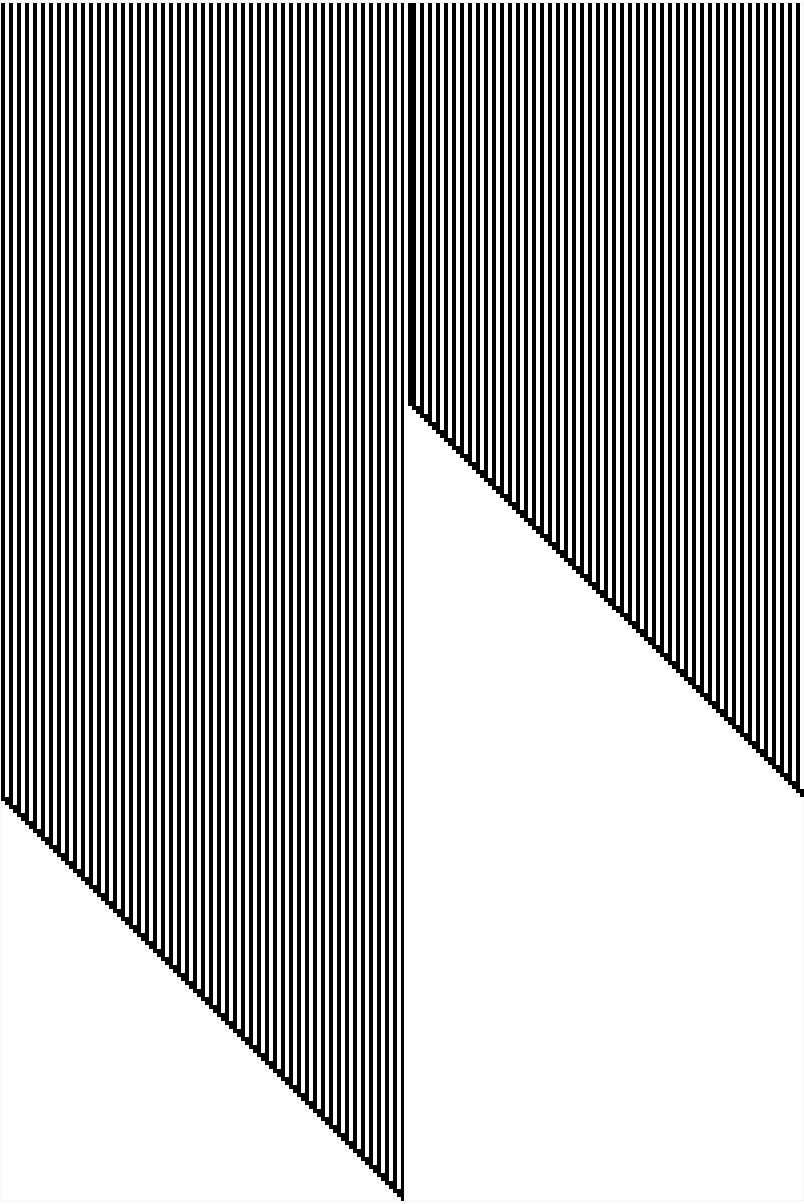
\includegraphics[width=\textwidth]{q3-78}
    \caption{اتوماتای سلولی یک بعدی به طول ۲۰۱ با قانون ۷۸ و ۳۰۰ دوره زمانی، شرایط اولیه: تنها خانه‌ی ۱۰۱ روشن}
    \label{fig:q3-78}
  \end{minipage}
  \hfill
	\begin{minipage}[b]{0.3\textwidth}
	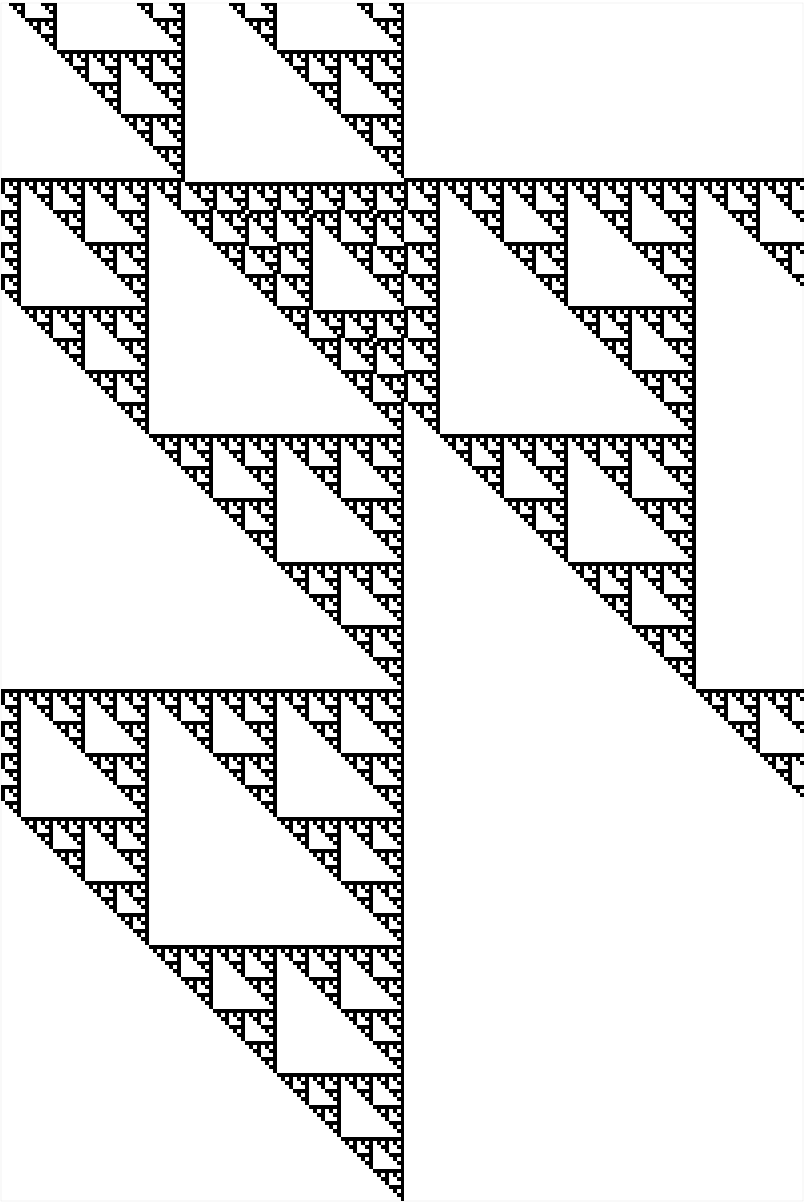
\includegraphics[width=\textwidth]{q3-102}
    \caption{اتوماتای سلولی یک بعدی به طول ۲۰۱ با قانون ۱۰۲ و ۳۰۰ دوره زمانی، شرایط اولیه: تنها خانه‌ی ۱۰۱ روشن}
	\label{fig:q3-102}
  \end{minipage}
  \hfill
\end{figure}
\begin{figure}[!tbp]
  \begin{minipage}[b]{0.3\textwidth}
    
\includegraphics[width=\textwidth]{q3-106}
    \caption{اتوماتای سلولی یک بعدی به طول ۲۰۱ با قانون ۱۰۶ و ۳۰۰ دوره زمانی، شرایط اولیه: تنها خانه‌ی ۱۰۱ روشن}
    \label{fig:q3-106}
  \end{minipage}
  \hfill
  \begin{minipage}[b]{0.3\textwidth}
    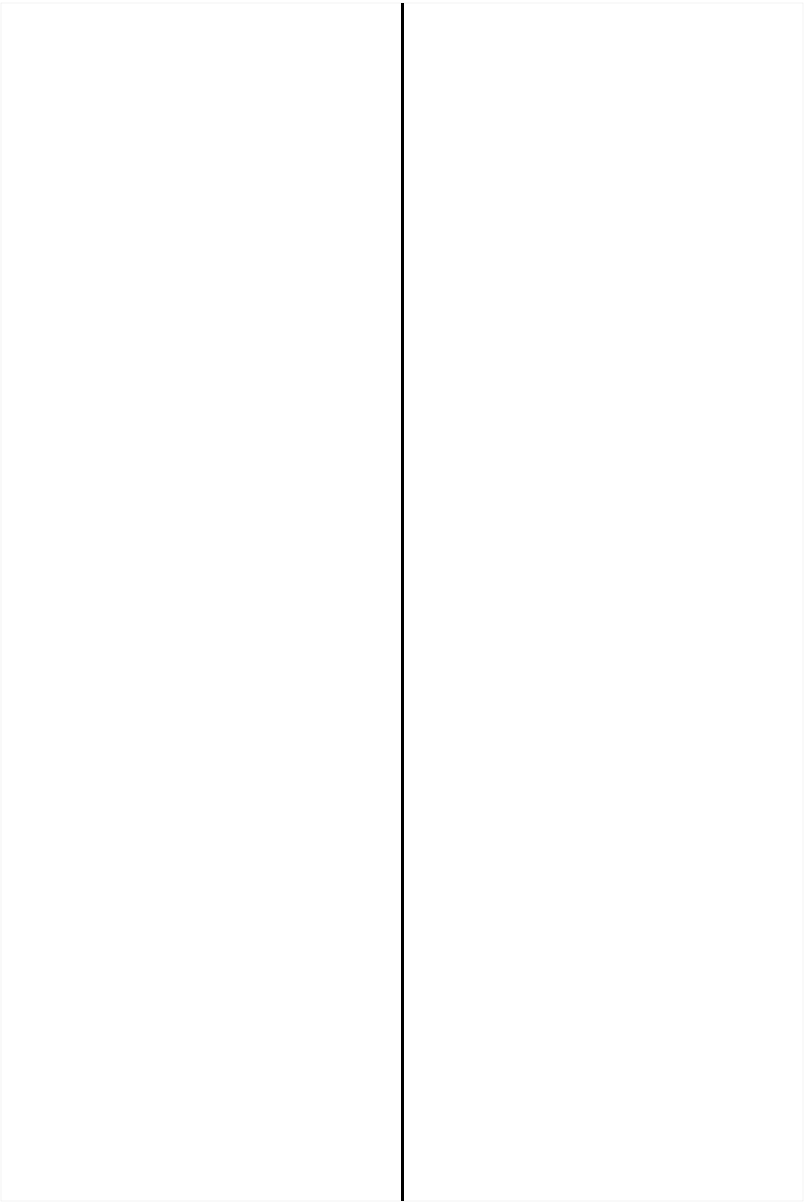
\includegraphics[width=\textwidth]{q3-108}
    \caption{اتوماتای سلولی یک بعدی به طول ۲۰۱ با قانون ۱۰۸ و ۳۰۰ دوره زمانی، شرایط اولیه: تنها خانه‌ی ۱۰۱ روشن}
    \label{fig:q3-108}
  \end{minipage}
  \hfill
	\begin{minipage}[b]{0.3\textwidth}
	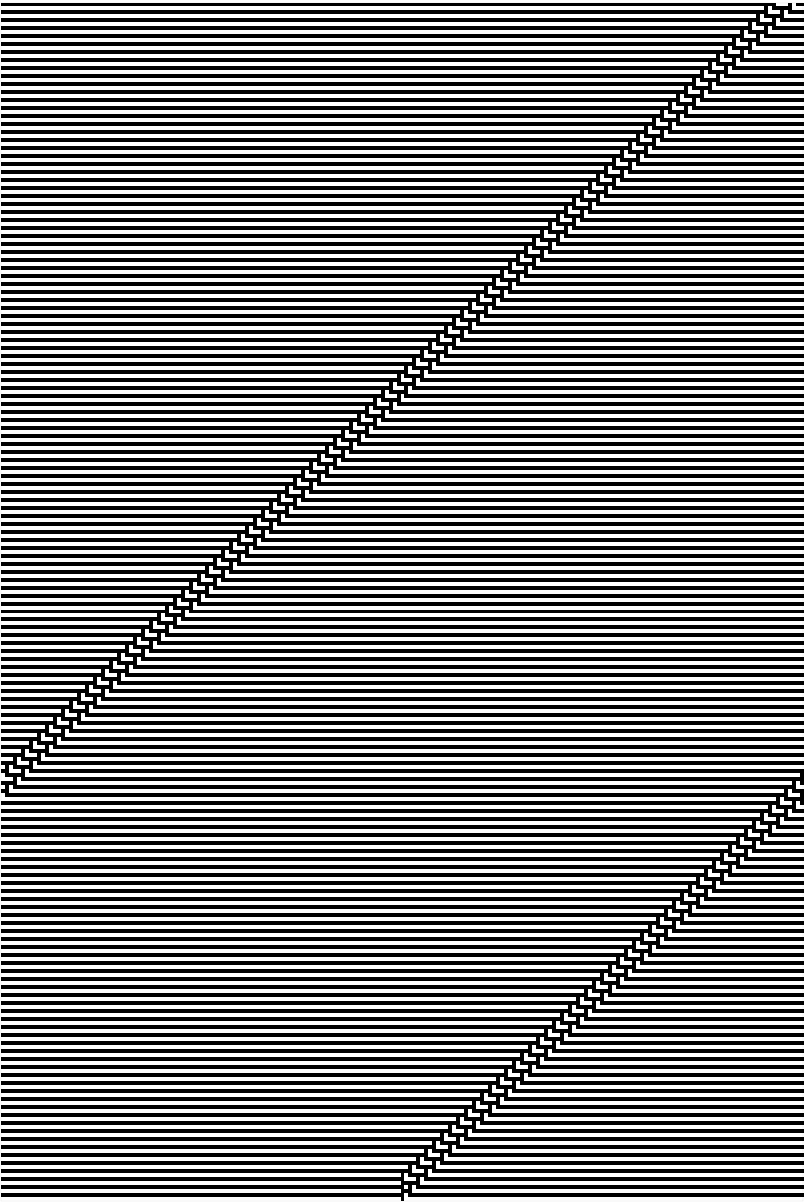
\includegraphics[width=\textwidth]{q3-111}
    \caption{اتوماتای سلولی یک بعدی به طول ۲۰۱ با قانون ۱۱۱ و ۳۰۰ دوره زمانی، شرایط اولیه: تنها خانه‌ی ۱۰۱ روشن}
	\label{fig:q3-111}
  \end{minipage}
  \hfill
\end{figure}
\begin{figure}[!tbp]
  \begin{minipage}[b]{0.3\textwidth}
    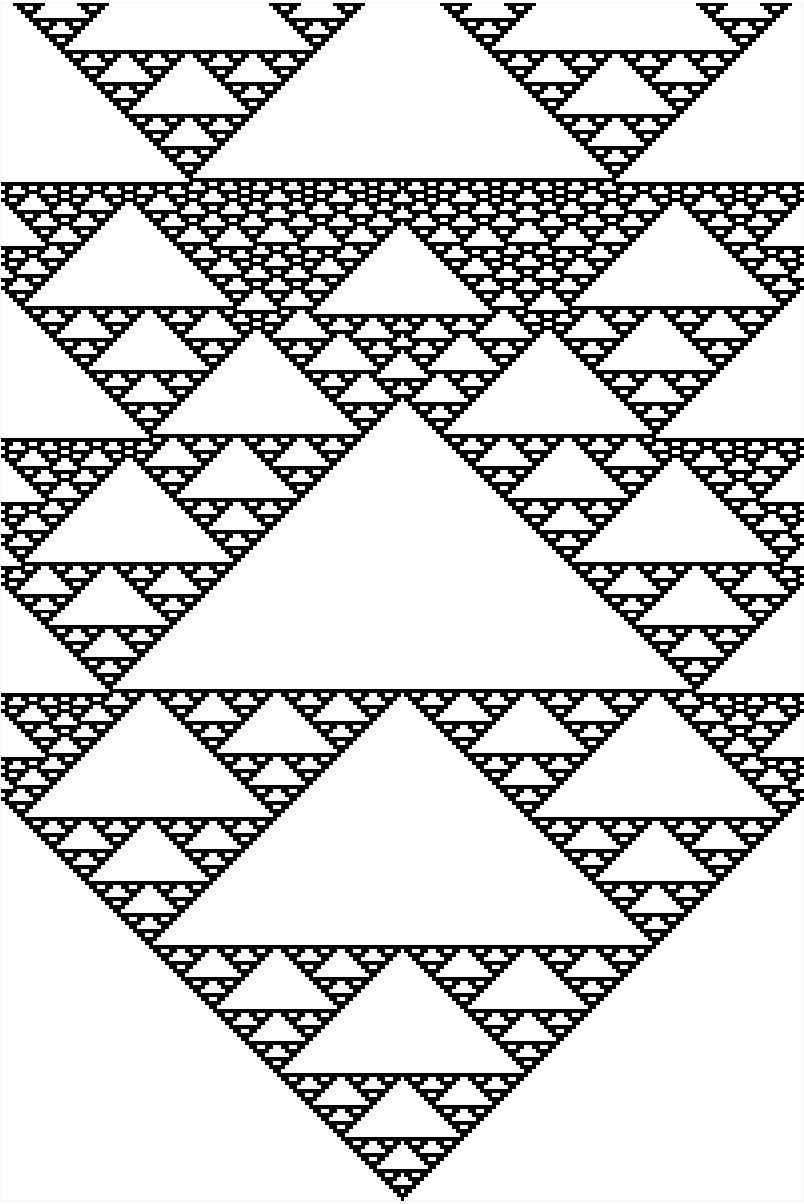
\includegraphics[width=\textwidth]{q3-126}
    \caption{اتوماتای سلولی یک بعدی به طول ۲۰۱ با قانون ۱۲۶ و ۳۰۰ دوره زمانی، شرایط اولیه: تنها خانه‌ی ۱۰۱ روشن}
    \label{fig:q3-126}
  \end{minipage}
  \hfill
  \begin{minipage}[b]{0.3\textwidth}
    
\includegraphics[width=\textwidth]{q3-238}
    \caption{اتوماتای سلولی یک بعدی به طول ۲۰۱ با قانون ۲۳۸ و ۳۰۰ دوره زمانی، شرایط اولیه: تنها خانه‌ی ۱۰۱ روشن}
    \label{fig:q3-238}
  \end{minipage}
  \hfill
\end{figure}

\begin{figure}[!tbp]
  \begin{minipage}[b]{0.3\textwidth}
    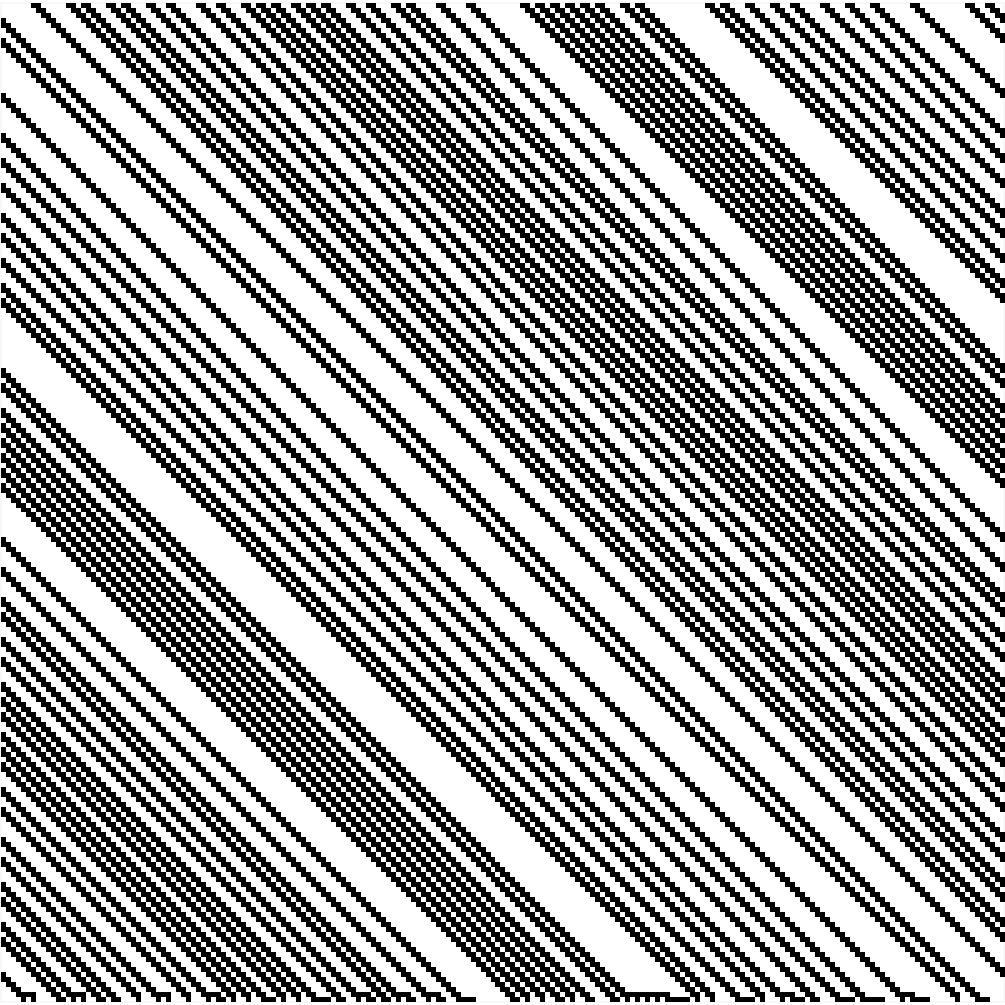
\includegraphics[width=\textwidth]{q3-46-rand}
    \caption{اتوماتای سلولی یک بعدی به طول ۲۰۱ با قانون ۴۶ و ۲۰۰ دوره زمانی، شرایط اولیه‌ی تصادفی}
    \label{fig:q3-46-rand}
  \end{minipage}
  \hfill
  \begin{minipage}[b]{0.3\textwidth}
    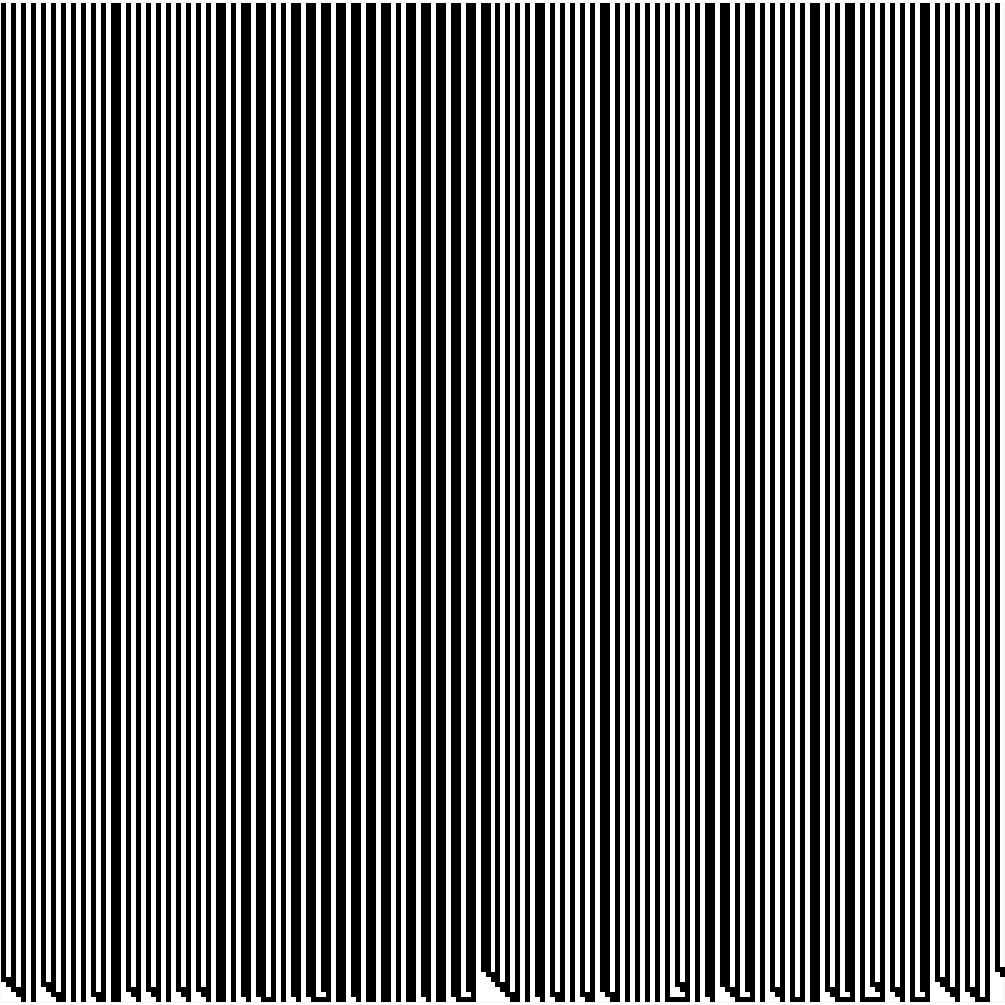
\includegraphics[width=\textwidth]{q3-78-rand}
    \caption{اتوماتای سلولی یک بعدی به طول ۲۰۱ با قانون ۷۸ و ۲۰۰ دوره زمانی، شرایط اولیه‌ی تصادفی}
    \label{fig:q3-78-rand}
  \end{minipage}
  \hfill
	\begin{minipage}[b]{0.3\textwidth}
	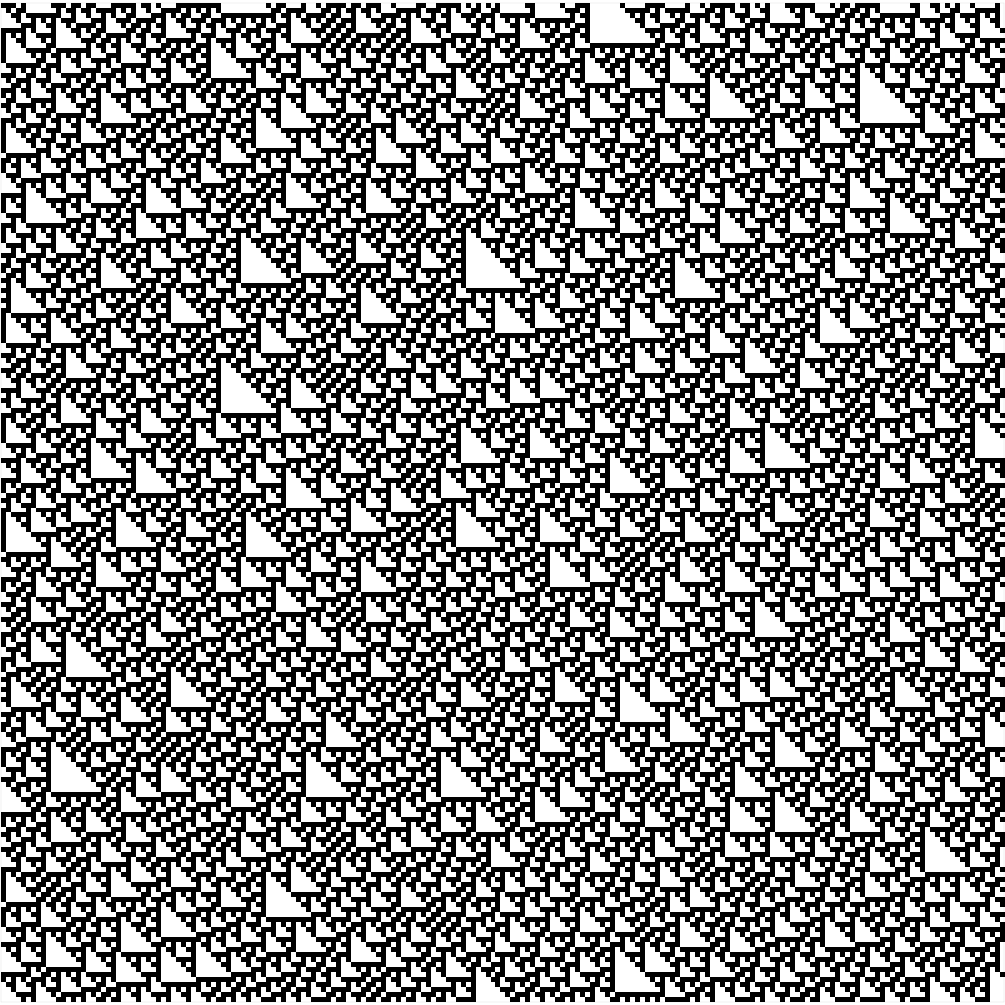
\includegraphics[width=\textwidth]{q3-102-rand}
    \caption{اتوماتای سلولی یک بعدی به طول ۲۰۱ با قانون ۱۰۲ و ۲۰۰ دوره زمانی، شرایط اولیه‌ی تصادفی}
	\label{fig:q3-102-rand}
  \end{minipage}
  \hfill
\end{figure}
\begin{figure}[!tbp]
  \begin{minipage}[b]{0.3\textwidth}
    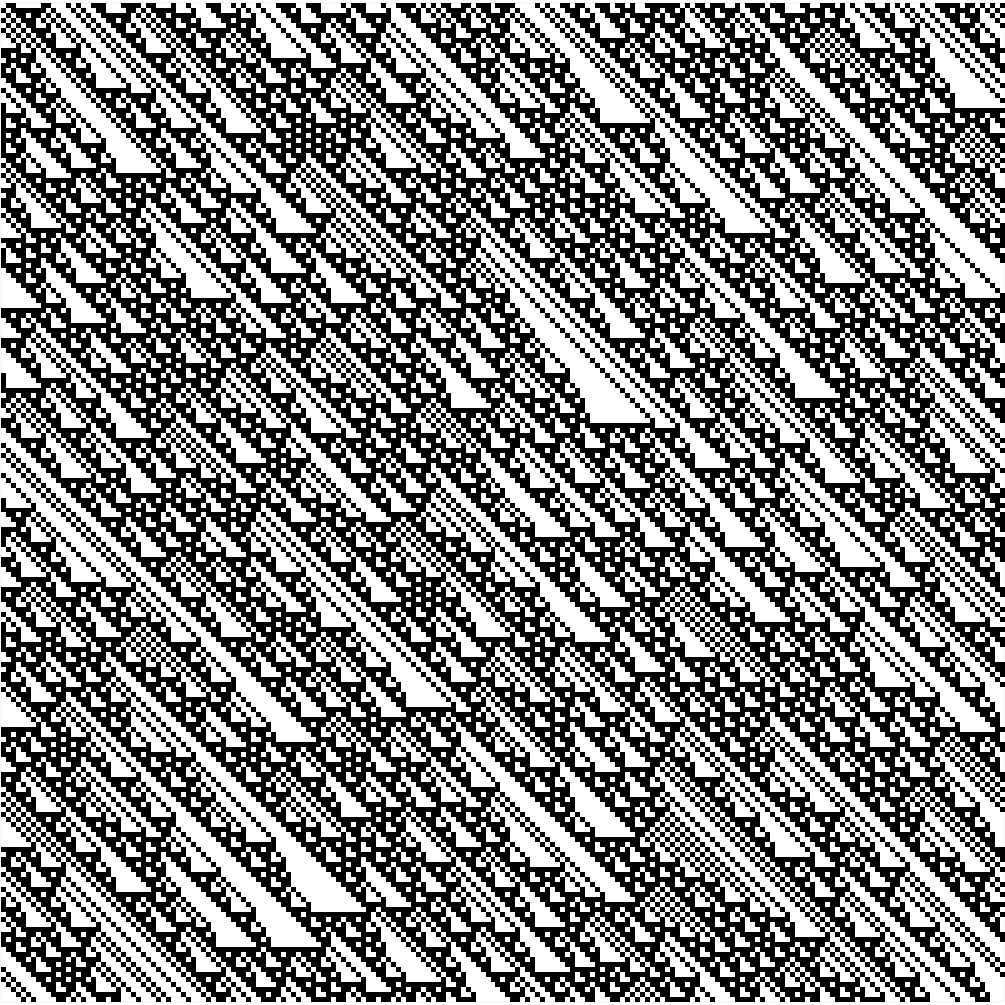
\includegraphics[width=\textwidth]{q3-106-rand}
    \caption{اتوماتای سلولی یک بعدی به طول ۲۰۱ با قانون ۱۰۶ و ۲۰۰ دوره زمانی، شرایط اولیه‌ی تصادفی}
    \label{fig:q3-106-rand}
  \end{minipage}
  \hfill
  \begin{minipage}[b]{0.3\textwidth}
    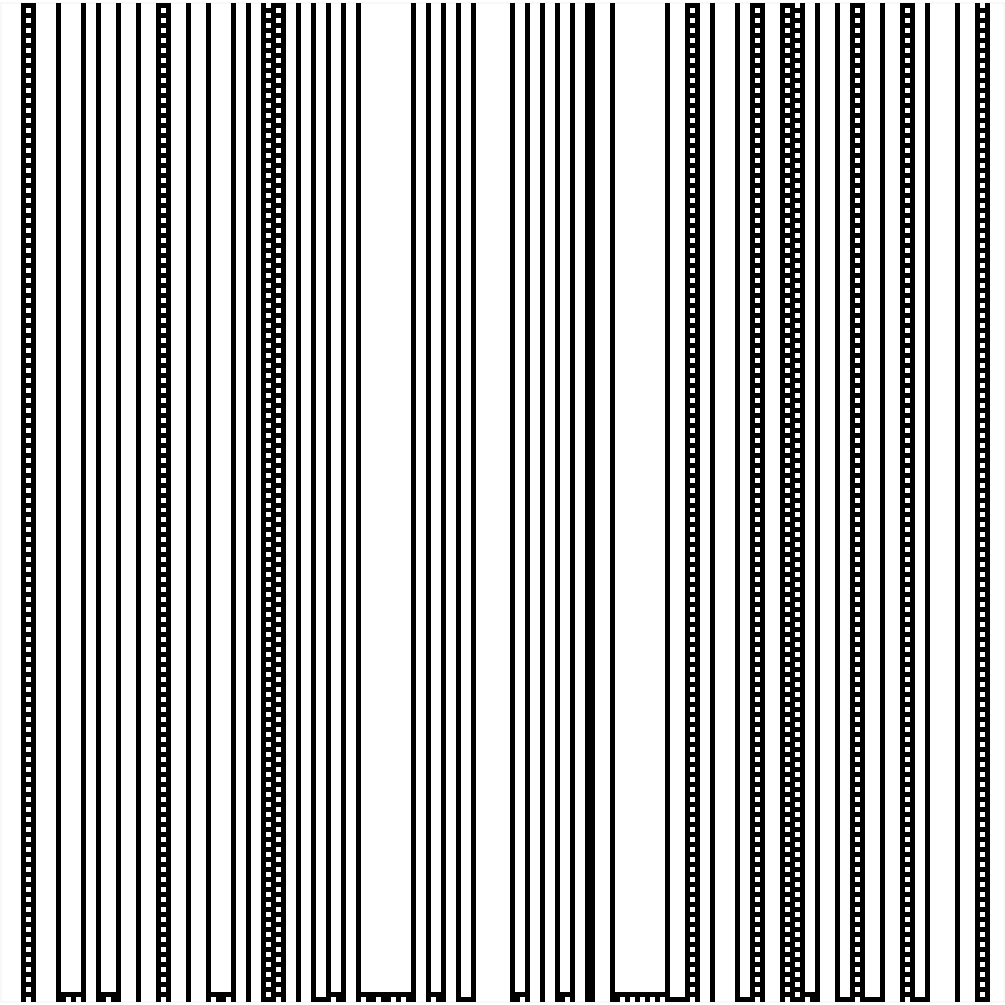
\includegraphics[width=\textwidth]{q3-108-rand}
    \caption{اتوماتای سلولی یک بعدی به طول ۲۰۱ با قانون ۱۰۸ و ۲۰۰ دوره زمانی، شرایط اولیه‌ی تصادفی}
    \label{fig:q3-108-rand}
  \end{minipage}
  \hfill
	\begin{minipage}[b]{0.3\textwidth}
	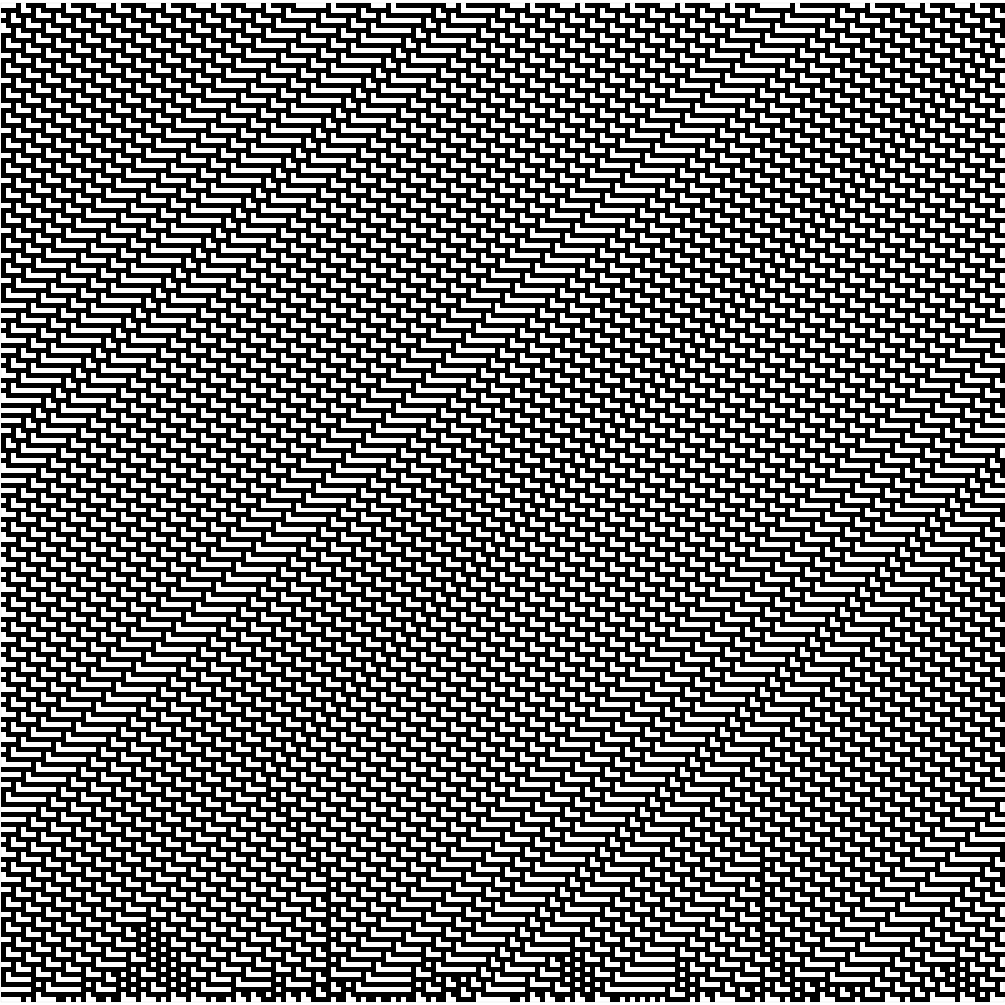
\includegraphics[width=\textwidth]{q3-111-rand}
    \caption{اتوماتای سلولی یک بعدی به طول ۲۰۱ با قانون ۱۱۱ و ۲۰۰ دوره زمانی، شرایط اولیه‌ی تصادفی}
	\label{fig:q3-111-rand}
  \end{minipage}
  \hfill
\end{figure}
\begin{figure}[!tbp]
  \begin{minipage}[b]{0.3\textwidth}
    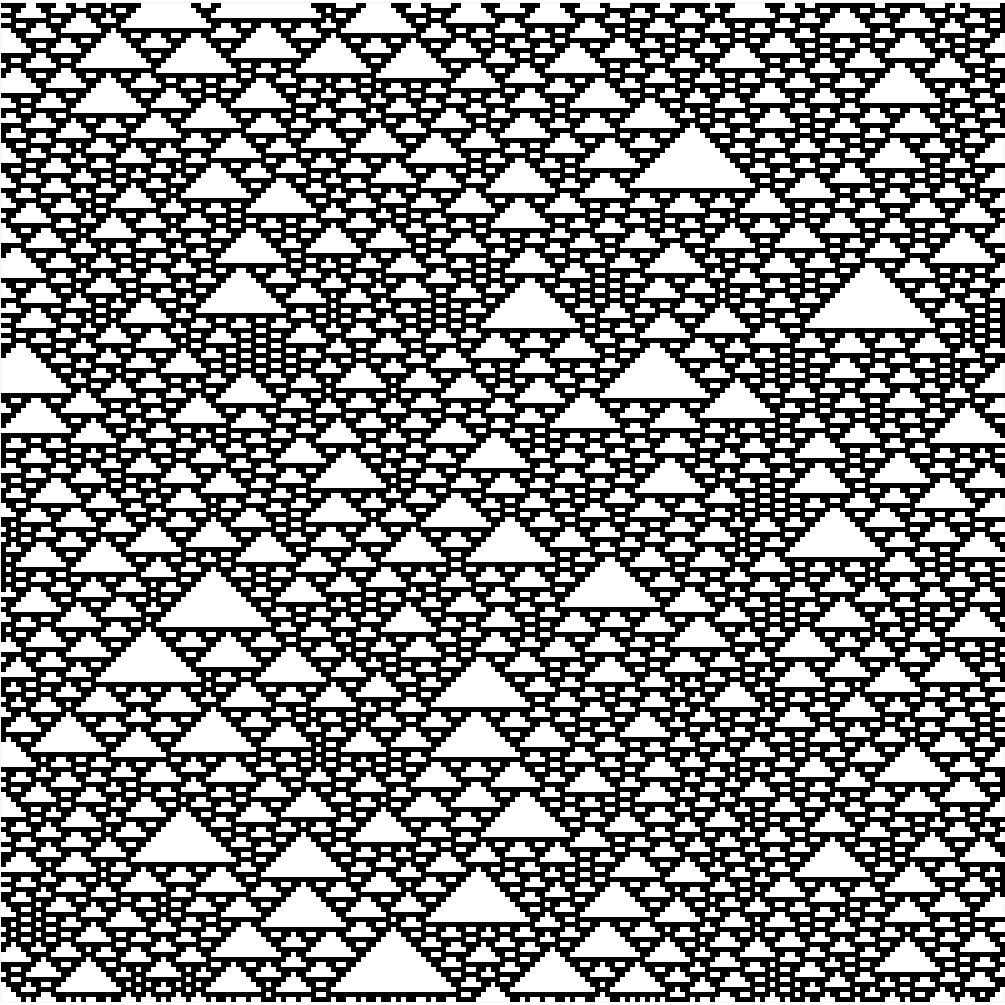
\includegraphics[width=\textwidth]{q3-126-rand}
    \caption{اتوماتای سلولی یک بعدی به طول ۲۰۱ با قانون ۱۲۶ و ۲۰۰ دوره زمانی، شرایط اولیه‌ی تصادفی}
    \label{fig:q3-126-rand}
  \end{minipage}
  \hfill
  \begin{minipage}[b]{0.3\textwidth}
    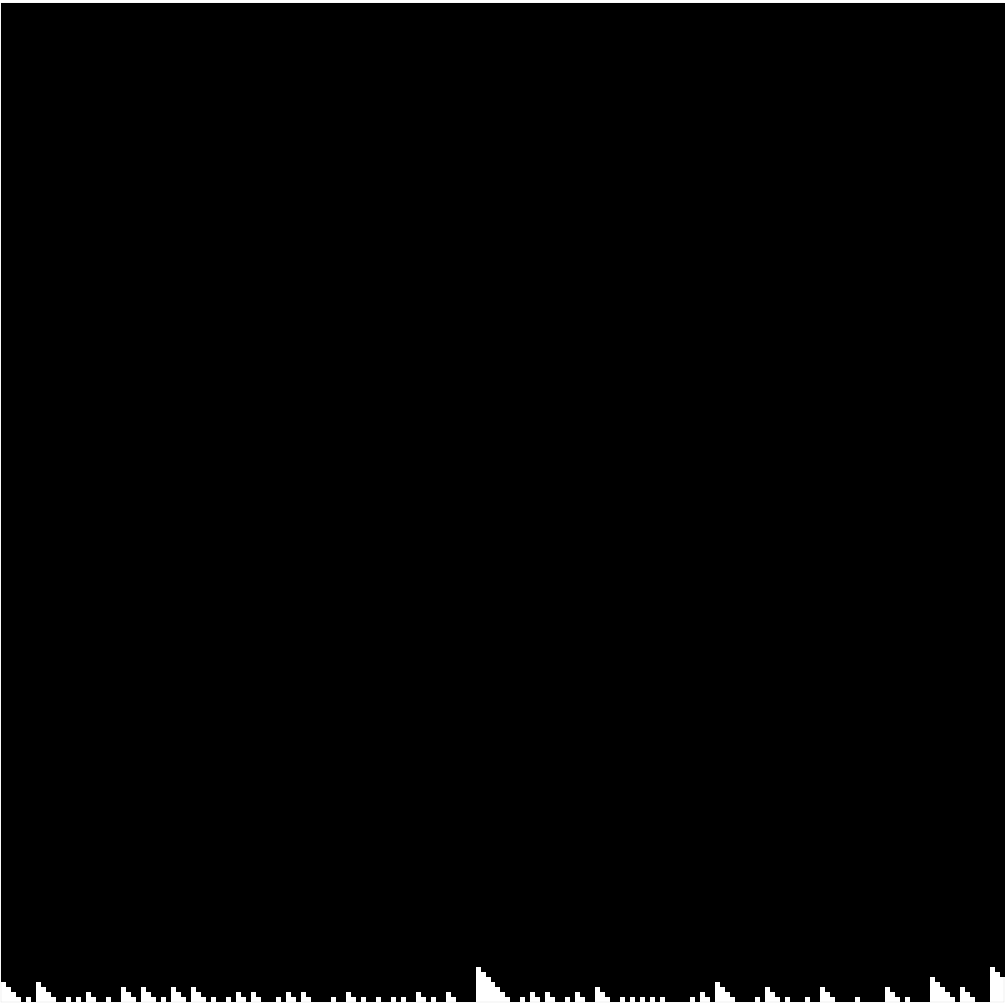
\includegraphics[width=\textwidth]{q3-238-rand}
    \caption{اتوماتای سلولی یک بعدی به طول ۲۰۱ با قانون ۲۳۸ و ۲۰۰ دوره زمانی، شرایط اولیه‌ی تصادفی}
    \label{fig:q3-238-rand}
  \end{minipage}
  \hfill
  \begin{minipage}[b]{0.3\textwidth}
    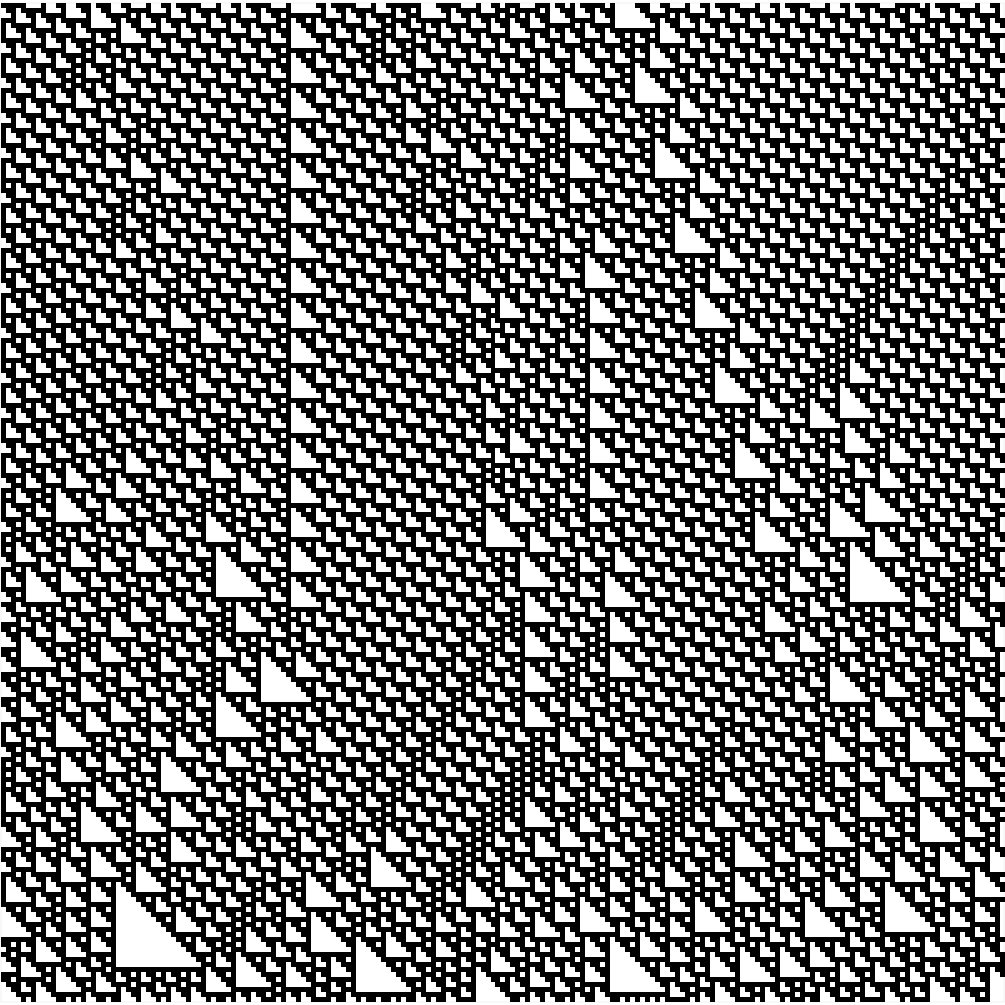
\includegraphics[width=\textwidth]{q3-110-rand}
    \caption{اتوماتای سلولی یک بعدی به طول ۲۰۱ با قانون ۱۱۰ و ۲۰۰ دوره زمانی، شرایط اولیه‌ی تصادفی}
    \label{fig:q3-110-rand}
  \end{minipage}
  \hfill
\end{figure}
\begin{figure}[!tbp]
  \begin{minipage}[b]{0.3\textwidth}
    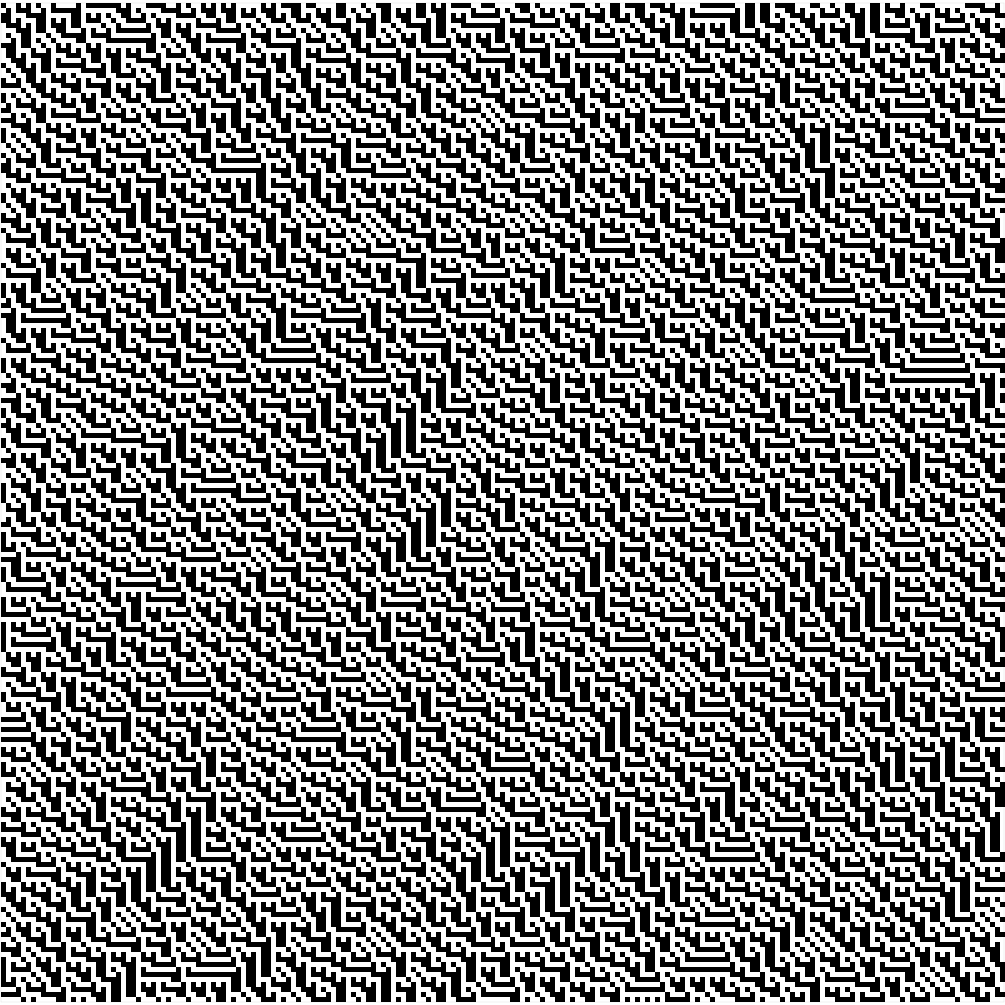
\includegraphics[width=\textwidth]{q3-75-rand}
    \caption{اتوماتای سلولی یک بعدی به طول ۲۰۱ با قانون ۷۵ و ۲۰۰ دوره زمانی، شرایط اولیه‌ی تصادفی}
    \label{fig:q3-75-rand}
  \end{minipage}
\end{figure}

\section{\textbf{\lr{Game of life}}}
\paragraph{}
در این قسمت نیز مشابه روندی که برای \lr{cellular automata} یک بعدی انجام دادیم، پیش می‌رویم. به این منظور کلاس \lr{GameOfLife} را در فایل \lr{automata.py} پیاد‌ه‌سازی می‌کنیم.\\
برای ساختن یک \lr{object} از این کلاس، به ۳ متغیر "طول"، "ارتفاع" و "شرایط اولیه" نیاز است. شرایط اولیه می‌تواند مقدار \lr{"rand"} داشته باشد که به معنای شرایط اولیه تصادفی است، یا می‌تواند یک رشته به شکل یک ماتریس باشد که خانه‌های روشن در آن با کارکتر \lr{"*"} مشخص شده‌اند و هم‌چنین می تواند لیستی از اندیس‌های خانه‌های روشن باشد. برای ذخیره‌سازی وضعیت سلول‌ها، از آرایه‌ای دو بعدی از متغیرهای \lr{boolean} استفاده می‌کنیم که خانه‌های روشن معادل با مقدار \lr{False} هستند.\\
برای انجام شبیه‌سازی باید تابع \lr{render} را با مقدار "زمانی" که می خواهیم آن را روشن بگذاریم، فراخوانی کنیم. روش کار این تابع به این صورت است که روی تک تک خانه‌های این لیست دو بعدی پیمایش می‌‌کند و اندیس‌های آن خانه‌ها را به تابع \lr{\_\_live\_neighbors\_\_} می‌فرستد تا تعداد همسایه‌های زنده‌ی آن سلول را به دست آوریم. این کار را هم به این صورت انجام می‌دهیم که روی لیست ۳ در ۳ همسایگی آن سلول پیمایش کرده و تعداد خانه‌های \lr{False} را می‌شماریم. بعد از آن که تعداد همسایه‌های زنده را به دست آوردیم، نوبت تعیین کردن وضعیت سلول در مرحله‌ی بعد می‌رسد. وضعیت جدید سلول بر اساس وضعیت پیشین سلول و تعداد همسایه‌های زنده‌ی آن تعیین می‌شود پس این دو مقدار را به تابع \lr{\_\_new\_state\_\_} می‌فرستیم و بر اساس قوانین تعیین شده در سوال، وضعیت جدید سلول را به دست می‌‌‌‌آوریم و به لیست جدیدمان اضافه می‌کنیم. در نهایت لیست کامل شده را، به لیست \lr{grids} اضافه می‌کنیم.\\
در نهایت برای نمایش دادن انیمیشن حاصل از تغییرات سلول‌ها، تابع \lr{animate} را باید فراخوانی کنیم. این تابع دو مقدار \lr{"interval"} و \lr{"name"} را می‌گیرد که اولی فاصله‌ی زمانی بین نمایش هر وضعیت را تعیین می‌کند و دومی اسم فایل ویدئوي ذخیره شده را. روش کار هم به این صورت است که ابتدا لیست دو بعدی هر مرحله را با استفاده از تابع \lr{imshow} از کتاب‌خانه‌ی \lr{matplotlib} به عکس تبدیل می‌کنیم و سپس عکس‌های به دست آمده را در یک لیست جدید ذخیره می‌کنیم. در نهایت این لیست را با تابع \lr{animation.ArtistAnimation} از کتاب‌خانه‌ی \lr{matplotlib}ِ، به انیمیشن تبدیل و سپس آن را ذخیره می‌کنیم.

\paragraph{}
با استفاده از تابع تشریح شده در بالا، شرایط اولیه را مطابق شکل‌های داده شده اعمال می‌کنیم و می‌گذاریم که به مدت ۱۰ واحد زمانی روشن بمانند. ویدئو‌های به دست آمده را در فولدر \lr{game\_of\_life\_animations} می‌توان مشاهده نمود.


\end{document}
